\chapter{Ponte di Wheatstone}
Il \textbf{ponte di Wheatstone} è un metodo di misura per \textbf{resistenze di ordine medio}.\\ \\
\begin{center}
    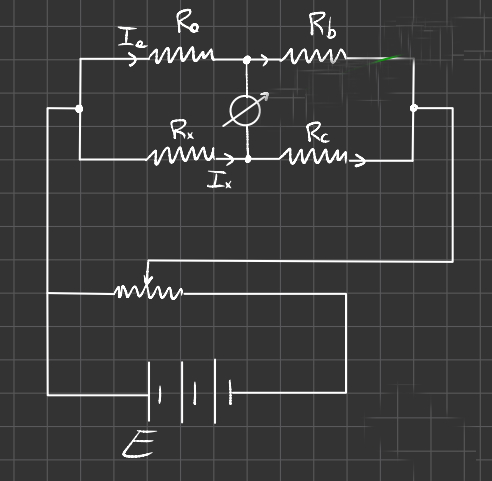
\includegraphics[width=.6\textwidth]{Images/figure5.png}
\end{center}
Esso è formato da:
\begin{itemize}
    \item $R_x$: \textbf{Resistenza Incognita}
    \item $R_a, R_b$: \textbf{Resistenze Fisse Note}
    \item $R_c$: \textbf{Resistenza Variabile Nota}
    \item E: \textbf{Batteria Nota}
\end{itemize}
Il ponte si dice in \textbf{equilibrio} quando è \textbf{nulla} la \textbf{corrente} nel \textbf{rilevatore di zero} e si ha:
\begin{equation*}
    \begin{rcases}
        R_a I_a = R_x I_x\\
        R_b I_a = R_c I_x
    \end{rcases}
    \implies 
    \frac{R_a}{R_b} = \frac{R_x}{R_c} \implies
\end{equation*}
\begin{equation*}
    \implies R_x = \frac{R_a}{R_b} R_c
\end{equation*}
Per far si che il \textbf{rilevatore di zero} non percepisca corrente vario $R_c$.
\section{Incertezza}
Indicando con $I_{min}$ la \textbf{minima corrente che il rilevatore di zero riesce a sentire}, scriveremo la relazione:
\begin{equation*}
    R_x = \frac{R_a}{R_b} \cdot R_c + R_s
\end{equation*}
Dove $R_s$ è un valore \textbf{aleatorio} a \textbf{media nulla} e \textbf{incertezza diversa da zero}.\\ \\
Quindi:
\begin{equation*}
    u^2_{R_x} = \underbrace{u^2_{\left(\frac{R_a}{R_b} \cdot R_c\right)}}_{\alpha} + \underbrace{u^2_{R_s}}_{\beta}
\end{equation*}
Dove $\alpha$ sarà:
\begin{equation*}
\begin{aligned}
    \dot{u}^2_{\left(\frac{R_a}{R_b} \cdot R_c\right)} &= \dot{u}^2_{R_a} + \dot{u}^2_{R_b} + \dot{u}^2_{R_c}\\
    {u}^2_{\left(\frac{R_a}{R_b} \cdot R_c\right)} &= \left(\frac{R_a}{R_b} \cdot R_c \right)^2 \cdot \dot{u}^2_{\left(\frac{R_a}{R_b} \cdot R_c\right)} = \\
    &= R^2_x \cdot \left(\dot{u}^2_{R_a} + \dot{u}^2_{R_b} + \dot{u}^2_{R_c}\right)
\end{aligned}
\end{equation*}
Mentre $\beta$ sarà:
\begin{equation*}
    \underbrace{dR_x}_{Rs} : d\lambda = \Delta R_x : \Delta \lambda \implies R_s = \frac{\Delta R_x}{\Delta \lambda} d\lambda
\end{equation*}
Dalla relazione caratteristica del ponte in \textbf{equilibrio} ho che:
\begin{equation*}
    \Delta (R_x) = \Delta \left(\frac{R_a}{R_b} R_c\right) = \frac{R_a}{R_b} \Delta R_c
\end{equation*}
Divido per $R_x$:
\begin{equation*}
    \frac{\Delta (R_x)}{R_x} = \frac{R_a}{R_b} \frac{\Delta R_c}{R_x} = \frac{R_a}{R_b} \frac{\Delta R_c}{ \frac{R_a}{R_b} R_c} = \frac{\Delta R_c}{R_c}
\end{equation*}
Quindi sostituendo $\Delta R_x = \Delta R_c \frac{R_x}{R_c}$ a $£
R_s$ otteniamo:
\begin{equation*}
    R_s = \Delta R_c \cdot \frac{d \lambda}{\Delta \lambda} \cdot \underbrace{\frac{R_x}{R_c}}_{\approx 1} \approx \Delta R_c \frac{d \lambda}{\Delta \lambda}
\end{equation*}
Quindi la $R_s$ si può calcolare \textbf{variando significatamene} $R_c$ e valutando la corrispondente \textbf{deviazione} $\Delta \lambda$ del rilevatore.
\section{Tecnica della Doppia Pesata}
Si effettuano due misure su $R_x$, \textbf{scambiando} $R_a$ e $R_b$ di posto:
\begin{equation*}
    \begin{dcases}
        Prima \ misura: \ R_x = \frac{R_a}{R_b} R_c\\
        Seconda \ misura: \ R_x = \frac{R_a}{R_b} R'_c
    \end{dcases}
\end{equation*}
Dove:
\begin{equation*}
    R'_c = R_c + r, \quad con \ r<< R_c
\end{equation*}
Consideriamo ora la \textbf{moltiplicazione} tra le due misurazioni:
\begin{equation*}
    R_x * R_x = R_c * R'_c = R_c^2 \left(1 + \frac{r}{R_c}\right)
\end{equation*}
Quindi:
\begin{equation*}
    R_x = R_c \sqrt{1 + \frac{r}{R_c}} \approx R_c \left(1 + \frac{r}{2R_c}\right) = R_c\left(\frac{2R_c + r}{2R_c}\right)
\end{equation*}
Questo metodo lega la \textbf{resistenza incognita} $R_x$ alla \textbf{resistenza campione} $R_c$ delle due misure, rendendola \textbf{indipendente} dalle incertezze di $R_a$ e $R_b$.
\section{Tecnica della Sostituzione}
Questo metodo viene utilizzato per la misura del \textbf{rapporto} di resistenze \textbf{simili tra loro}:
\begin{equation*}
    \frac{R_y}{R_x} \quad con \quad R_x \approx R_y
\end{equation*}
Dove:
\begin{equation*}
\begin{rcases}
    R_x = \frac{R_a}{R_b} R_c\\
    R_y = \frac{R_a}{R_b} R'_c
\end{rcases}
\implies \frac{R_y}{R_x} = \frac{R'_c}{R_c} = \frac{R_c + r}{R_c} = 1 + \frac{r}{R_c}
\end{equation*}
Così anche in questo caso ci siamo \textbf{sganciati dalla dipendenza} dell'incertezza di $R_a$ e $R_b$.
\section{Half-Bridge e Full-Bridge}
In questa conformazione, anzichè mettere il ponte in \textbf{equilibrio}, lo mettiamo in queste condizioni:
\begin{center}
    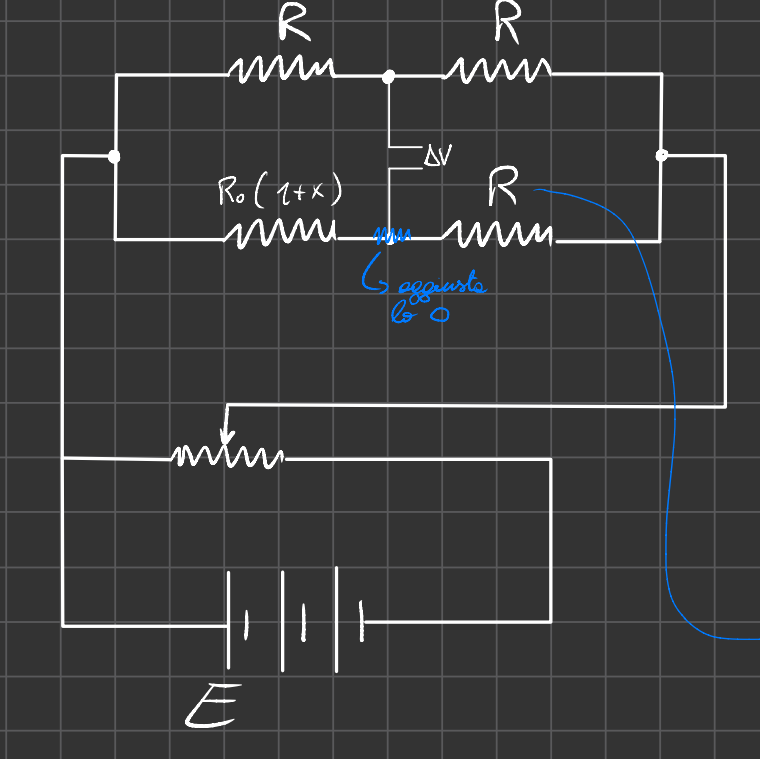
\includegraphics[width=.6\textwidth]{Images/figure6.png}
\end{center}
E misuriamo:
\begin{equation*}
    \Delta V \approx \frac{E}{4} X, \ se \ X << 1
\end{equation*}
Se ora mettessi $R(1-X)$ sulla resistenza con la linea blu otterrei la configurazione \textbf{Half-Bridge}, dove vale:
\begin{equation*}
    \Delta V = \frac{E}{2}X 
\end{equation*}
Che è valida anche per \textbf{grandi X}.\\ \\
Se ora mettessi $R(1 - X)$ su $R_a$ e $R( 1 + X )$ su $R_b$ otterrei il \textbf{Full-Bridge}, dove vale:
\begin{equation*}
    \Delta V = E \cdot X
\end{equation*}
